
\documentclass[letterpaper,hide notes,xcolor={table,svgnames},pdftex,10pt]{beamer}
\def\showexamples{t}

\usecolortheme{crane}
\setbeamertemplate{navigation symbols}{}

\usetheme{MyPittsburgh}
\usepackage{hyperref}
\usepackage{graphicx,xspace}
\usepackage[normalem]{ulem}
\usepackage{multicol}
\usepackage{amsmath,amssymb,amsthm,graphicx,xspace}
\newcommand\SF[1]{$\bigstar$\footnote{SF: #1}}

\usepackage[sfdefault,lf]{carlito}
\usepackage[T1]{fontenc}
\usepackage[scaled]{beramono}
\usepackage{tikzpagenodes}
\newcommand{\Rplus}{\protect\hspace{-.1em}\protect\raisebox{.35ex}{\small{\small\textbf{+}}}}
\newcommand{\Cpp}{\mbox{C\Rplus\Rplus}\xspace}

\newcounter{tmpnumSlide}
\newcounter{tmpnumNote}

\newcommand\mnote[1]{%
	\addtocounter{tmpnumSlide}{1}
	\ifdefined\showcues {~\tiny\fbox{\arabic{tmpnumSlide}}}\fi
	\note{\setlength{\parskip}{1ex}\addtocounter{tmpnumNote}{1}\textbf{\Large \arabic{tmpnumNote}:} {#1\par}}}

\newcommand\mmnote[1]{\note{\setlength{\parskip}{1ex}#1\par}}


\newcommand\mquestion[2]{{~\color{red}\fbox{?}}\note{\setlength{\parskip}{1ex}\par{\Large \textbf{?}} #1} \note{\setlength{\parskip}{1ex}\par{\Large \textbf{A}} #2\par}\ifdefined \presentationonly \pause \fi}

\newcommand\blackboard[1]{%
	\ifdefined   \showblackboard
		{#1}
	\else {\begin{center} \fbox{\colorbox{blue!30}{%
						\begin{minipage}{.95\linewidth}%
							\hspace{\stretch{1}} Some space intentionally left blank; done at the blackboard.%
						\end{minipage}}}\end{center}}%
	\fi%
}

\usepackage{listings}
\lstset{%
	keywordstyle=\bfseries,
	aboveskip=15pt,
	belowskip=15pt,
	captionpos=b,
	identifierstyle=\ttfamily,
	frame=lines,
	numbers=left, basicstyle=\scriptsize, numberstyle=\tiny, stepnumber=0, numbersep=2pt}

\usepackage{siunitx}
\newcommand\sius[1]{\num[group-separator = {,}]{#1}\si{\micro\second}}
\newcommand\sims[1]{\num[group-separator = {,}]{#1}\si{\milli\second}}
\newcommand\sins[1]{\num[group-separator = {,}]{#1}\si{\nano\second}}
\sisetup{group-separator = {,}, group-digits = true}

%% -------------------- tikz --------------------
\usepackage{tikz}
\usetikzlibrary{positioning}
\usetikzlibrary{arrows,backgrounds,automata,decorations.shapes,decorations.pathmorphing,decorations.markings,decorations.text}

\tikzstyle{place}=[circle,draw=blue!50,fill=blue!20,thick, inner sep=0pt,minimum size=6mm]
\tikzstyle{transition}=[rectangle,draw=black!50,fill=black!20,thick, inner sep=0pt,minimum size=4mm]

\tikzstyle{block}=[rectangle,draw=black, thick, inner sep=5pt]
\tikzstyle{bullet}=[circle,draw=black, fill=black, thin, inner sep=2pt]

\tikzstyle{pre}=[<-,shorten <=1pt,>=stealth',semithick]
\tikzstyle{post}=[->,shorten >=1pt,>=stealth',semithick]
\tikzstyle{bi}=[<->,shorten >=1pt,shorten <=1pt, >=stealth',semithick]

\tikzstyle{mut}=[-,>=stealth',semithick]

\tikzstyle{treereset}=[dashed,->, shorten >=1pt,>=stealth',thin]

\usepackage{ifmtarg}
\usepackage{xifthen}
\makeatletter
% new counter to now which frame it is within the sequence
\newcounter{multiframecounter}
% initialize buffer for previously used frame title
\gdef\lastframetitle{\textit{undefined}}
% new environment for a multi-frame
\newenvironment{multiframe}[1][]{%
	\ifthenelse{\isempty{#1}}{%
		% if no frame title was set via optional parameter,
		% only increase sequence counter by 1
		\addtocounter{multiframecounter}{1}%
	}{%
		% new frame title has been provided, thus
		% reset sequence counter to 1 and buffer frame title for later use
		\setcounter{multiframecounter}{1}%
		\gdef\lastframetitle{#1}%
	}%
	% start conventional frame environment and
	% automatically set frame title followed by sequence counter
	\begin{frame}%
		\frametitle{\lastframetitle~{\normalfont(\arabic{multiframecounter})}}%
		}{%
	\end{frame}%
}
\makeatother

\makeatletter
\newdimen\tu@tmpa%
\newdimen\ydiffl%
\newdimen\xdiffl%
\newcommand\ydiff[2]{%
	\coordinate (tmpnamea) at (#1);%
	\coordinate (tmpnameb) at (#2);%
	\pgfextracty{\tu@tmpa}{\pgfpointanchor{tmpnamea}{center}}%
	\pgfextracty{\ydiffl}{\pgfpointanchor{tmpnameb}{center}}%
	\advance\ydiffl by -\tu@tmpa%
}
\newcommand\xdiff[2]{%
	\coordinate (tmpnamea) at (#1);%
	\coordinate (tmpnameb) at (#2);%
	\pgfextractx{\tu@tmpa}{\pgfpointanchor{tmpnamea}{center}}%
	\pgfextractx{\xdiffl}{\pgfpointanchor{tmpnameb}{center}}%
	\advance\xdiffl by -\tu@tmpa%
}
\makeatother
\newcommand{\copyrightbox}[3][r]{%
	\begin{tikzpicture}%
		\node[inner sep=0pt,minimum size=2em](ciimage){#2};
		\usefont{OT1}{phv}{n}{n}\fontsize{4}{4}\selectfont
		\ydiff{ciimage.south}{ciimage.north}
		\xdiff{ciimage.west}{ciimage.east}
		\ifthenelse{\equal{#1}{r}}{%
			\node[inner sep=0pt,right=1ex of ciimage.south east,anchor=north west,rotate=90]%
			{\raggedleft\color{black!50}\parbox{\the\ydiffl}{\raggedright{}#3}};%
		}{%
			\ifthenelse{\equal{#1}{l}}{%
				\node[inner sep=0pt,right=1ex of ciimage.south west,anchor=south west,rotate=90]%
				{\raggedleft\color{black!50}\parbox{\the\ydiffl}{\raggedright{}#3}};%
			}{%
				\node[inner sep=0pt,below=1ex of ciimage.south west,anchor=north west]%
				{\raggedleft\color{black!50}\parbox{\the\xdiffl}{\raggedright{}#3}};%
			}
		}
	\end{tikzpicture}
}


%% --------------------

%\usepackage[excludeor]{everyhook}
%\PushPreHook{par}{\setbox0=\lastbox\llap{MUH}}\box0}

%\vspace*{\stretch{1}

%\setbox0=\lastbox \llap{\textbullet\enskip}\box0}

\setlength{\parskip}{\fill}

\newcommand\noskips{\setlength{\parskip}{1ex}}
\newcommand\doskips{\setlength{\parskip}{\fill}}

\newcommand\xx{\par\vspace*{\stretch{1}}\par}
\newcommand\xxs{\par\vspace*{2ex}\par}
\newcommand\tuple[1]{\langle #1 \rangle}
\newcommand\code[1]{{\sf \footnotesize #1}}
\newcommand\ex[1]{\uline{Example:} \ifdefined \presentationonly \pause \fi
	\ifdefined\showexamples#1\xspace\else{\uline{\hspace*{2cm}}}\fi}

\newcommand\ceil[1]{\lceil #1 \rceil}


\AtBeginSection[]
{
	\begin{frame}
		\frametitle{Outline}
		\tableofcontents[currentsection]
	\end{frame}
}



\pgfdeclarelayer{edgelayer}
\pgfdeclarelayer{nodelayer}
\pgfsetlayers{edgelayer,nodelayer,main}

\tikzstyle{none}=[inner sep=0pt]
\tikzstyle{rn}=[circle,fill=Red,draw=Black,line width=0.8 pt]
\tikzstyle{gn}=[circle,fill=Lime,draw=Black,line width=0.8 pt]
\tikzstyle{yn}=[circle,fill=Yellow,draw=Black,line width=0.8 pt]
\tikzstyle{empty}=[circle,fill=White,draw=Black]
\tikzstyle{bw} = [rectangle, draw, fill=blue!20,
text width=4em, text centered, rounded corners, minimum height=2em]

\newcommand{\CcNote}[1]{% longname
	This work is licensed under the \textit{Creative Commons #1 3.0 License}.%
}
\newcommand{\CcImageBy}[1]{%
	\includegraphics[scale=#1]{creative_commons/cc_by_30.pdf}%
}
\newcommand{\CcImageSa}[1]{%
	\includegraphics[scale=#1]{creative_commons/cc_sa_30.pdf}%
}
\newcommand{\CcImageNc}[1]{%
	\includegraphics[scale=#1]{creative_commons/cc_nc_30.pdf}%
}
\newcommand{\CcGroupBySa}[2]{% zoom, gap
	\CcImageBy{#1}\hspace*{#2}\CcImageNc{#1}\hspace*{#2}\CcImageSa{#1}%
}
\newcommand{\CcLongnameByNcSa}{Attribution-NonCommercial-ShareAlike}

\newenvironment{changemargin}[1]{% 
	\begin{list}{}{% 
		\setlength{\topsep}{0pt}% 
		\setlength{\leftmargin}{#1}% 
		\setlength{\rightmargin}{1em}
		\setlength{\listparindent}{\parindent}% 
		\setlength{\itemindent}{\parindent}% 
		      \setlength{\parsep}{\parskip}% 
		      }% 
		\item[]}{\end{list}}




\title{Lecture 27 --- Concurrency in File Systems }

\author{Jeff Zarnett \\ \small \texttt{jzarnett@uwaterloo.ca}}
\institute{Department of Electrical and Computer Engineering \\
	University of Waterloo}
\date{\today}


\begin{document}

\begin{frame}
	\titlepage

\end{frame}


\begin{frame}
\frametitle{Concurrency in File Systems}

We need to peel back the interface a bit and have at least a high-level understanding of their implementation.

File can be of arbitrary size (although in a particular file system there may be a limit).

They have to be allocated on disk according to some strategy.

\end{frame}

\begin{frame}
\frametitle{Contiguous Allocation}
Contiguous: a file occupies a set of contiguous blocks on disk. 

So a file is allocated, starting at block $b$ and is $n$ blocks in size, the file takes up blocks $b, b+1, b+2, ..., b+(n-1)$. 

This is advantageous, because if we want to access block $b$ on disk, accessing $b+1$ requires no head movement, so seek time is nonexistent to minimal.

\end{frame}

\begin{frame}
\frametitle{Contiguous Allocation}

All that we need to maintain are $b$ and $n$: the start location and length of the file. 

Both sequential and direct access are very easy: the first block of a file is at $b$. 

To access a block $i$ at some offset into the file, it's at the base address $b$ plus $i$. 

Checking if the access is valid is also an easy operation: if $i < n$ then it is valid.

\end{frame}

\begin{frame}
\frametitle{Contiguous Allocation}

\begin{center}
	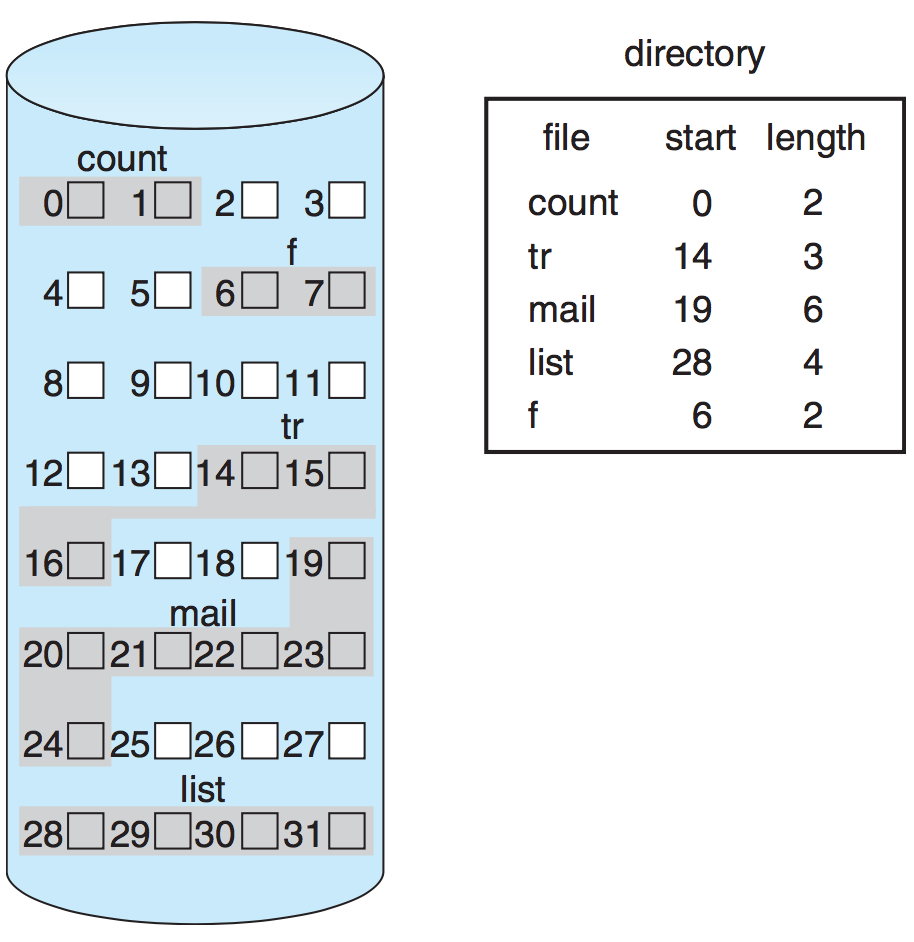
\includegraphics[width=0.6\textwidth]{images/disk-contiguous.png}
\end{center}

\end{frame}

\begin{frame}
\frametitle{Contiguous Allocation}


If we need a memory block of size $N$:\\
\quad (1) can we find a contiguous block of $N$ or greater to meet that allocation?\\
\quad (2) if there is more than one block, which one do we choose? 

As before, we suffer the problem of external fragmentation, plus a bit of internal fragmentation in the last block of the file. 

\end{frame}

\begin{frame}
\frametitle{Contiguous Allocation}

Another problem: how much space is a file going to take? 

If it is just a copy-paste operation, the copy is the same size as the original. 

When a user opens a new document, how big will it be? 

If we allocate too little space, we may be able to tack on space at the end, or that block may be allocated, forcing us to move the file and reallocate it. 

If the value we choose is too large, then significant space will be wasted for small files (and many files tend to be relatively small).

\end{frame}

\begin{frame}
\frametitle{Linked Allocation}

Linked allocation is a solution to the problems of contiguous allocation.

Instead of a file being all in consecutive blocks, we maintain a linked list of the blocks, and the blocks themselves may be located anywhere on the disk. 

The directory listing just has a pointer to the first and last blocks (head and tail of the linked list).

\end{frame}

\begin{frame}
\frametitle{Linked Allocation}

If a new file is created, it will be created with size zero and the head and tail pointers are null.

 When a new block is needed, it can come from anywhere and will just be added to the linked list. 
 
 Thus, compaction and relocation are not really an issue. 
 
 Unfortunately, however, accessing block $i$ of a file is no longer as simple as computing an offset from the first block; it requires following $i$ pointers (a pain).


\end{frame}

\begin{frame}
\frametitle{Linked Allocation}

\begin{center}
	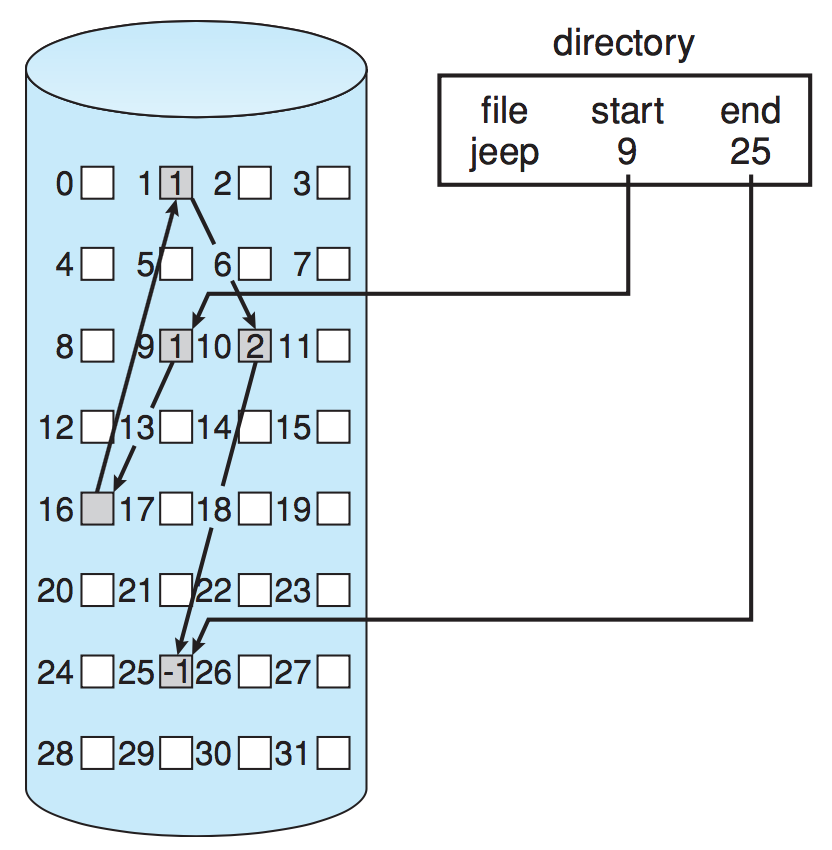
\includegraphics[width=0.6\textwidth]{images/disk-linked.png}
\end{center}

\end{frame}

\begin{frame}
\frametitle{Linked Allocation}

A possible solution to the problem of following so many pointers (and the overhead of maintaining so many) is to group up the blocks into \alert{clusters}.

A cluster is comprised of, say, four blocks. 

Then we waste less memory maintaining pointers and it improves disk accesses because there is less seeking back and forth to various disk locations.

\end{frame}

\begin{frame}
\frametitle{Indexed Allocation}

If we stuck to pure linked allocation, we still have the problem that accessing some part in the middle of the file is a pain.

We have to follow and retrieve a lot of pointers to the different blocks. 

The idea of indexed allocation is to take all the pointers and put them into one location: an index block. 


\end{frame}



\begin{frame}
\frametitle{Indexed Allocation}

So, the first block of the file contains a whole bunch of pointers. 

To get to block $i$, just go to index $i$ of the index block and we can get the location of block $i$ much more efficiently than we could in linked allocation. 

All pointers to blocks start as null, and when we add a new block, add its corresponding entry into the index block.

\end{frame}

\begin{frame}
\frametitle{Indexed Allocation}

\begin{center}
	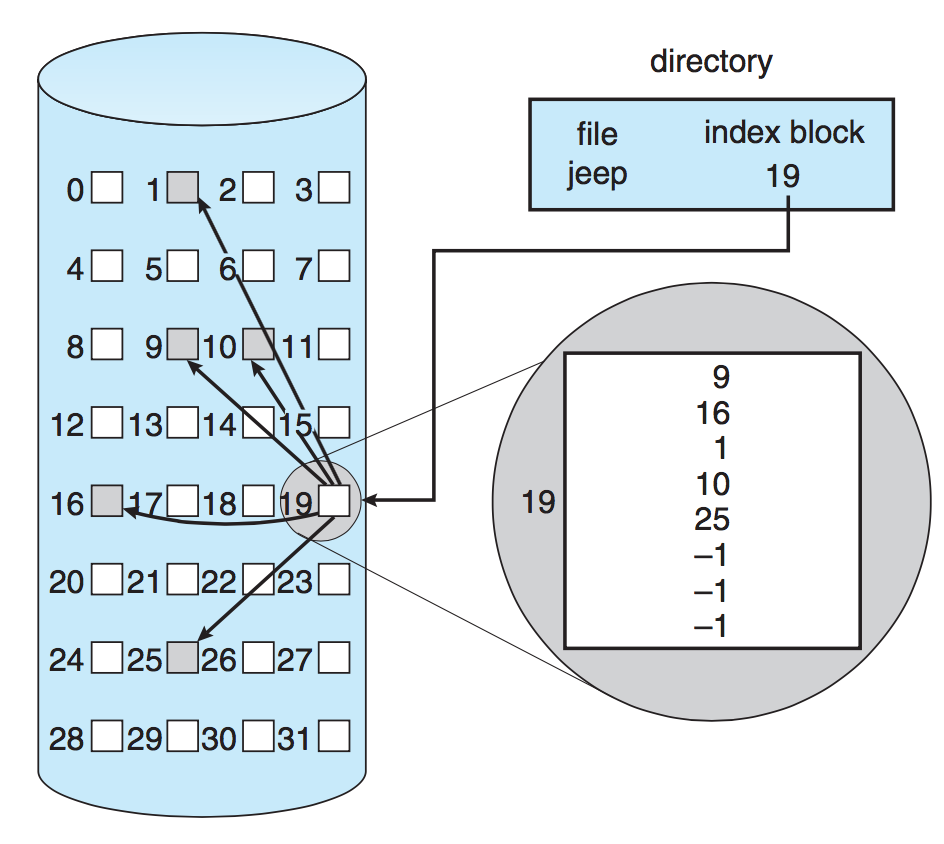
\includegraphics[width=0.6\textwidth]{images/disk-indexed.png}
\end{center}


\end{frame}

\begin{frame}
\frametitle{Block Size}

Like many of the other systems we have examined, there is a need to make a decision about the size of a block. 

If a file needs only 1-2 blocks, one whole block is allocated for the pointers which contains only 1-2 entries. 

That suggests we want the index to be small, but what if we need more pointers than fit into one block? There are a few mechanisms for this.


\end{frame}

\begin{frame}
\frametitle{Block Size}

What if we need more pointers than fit into one block?

\begin{enumerate}
	\item \textbf{Linked Scheme}
	\item \textbf{Multilevel Index}
	\item \textbf{Combined Scheme}
\end{enumerate}


\end{frame}

\begin{frame}
\frametitle{UNIX inodes}

A visual representation of an inode.

\begin{center}
	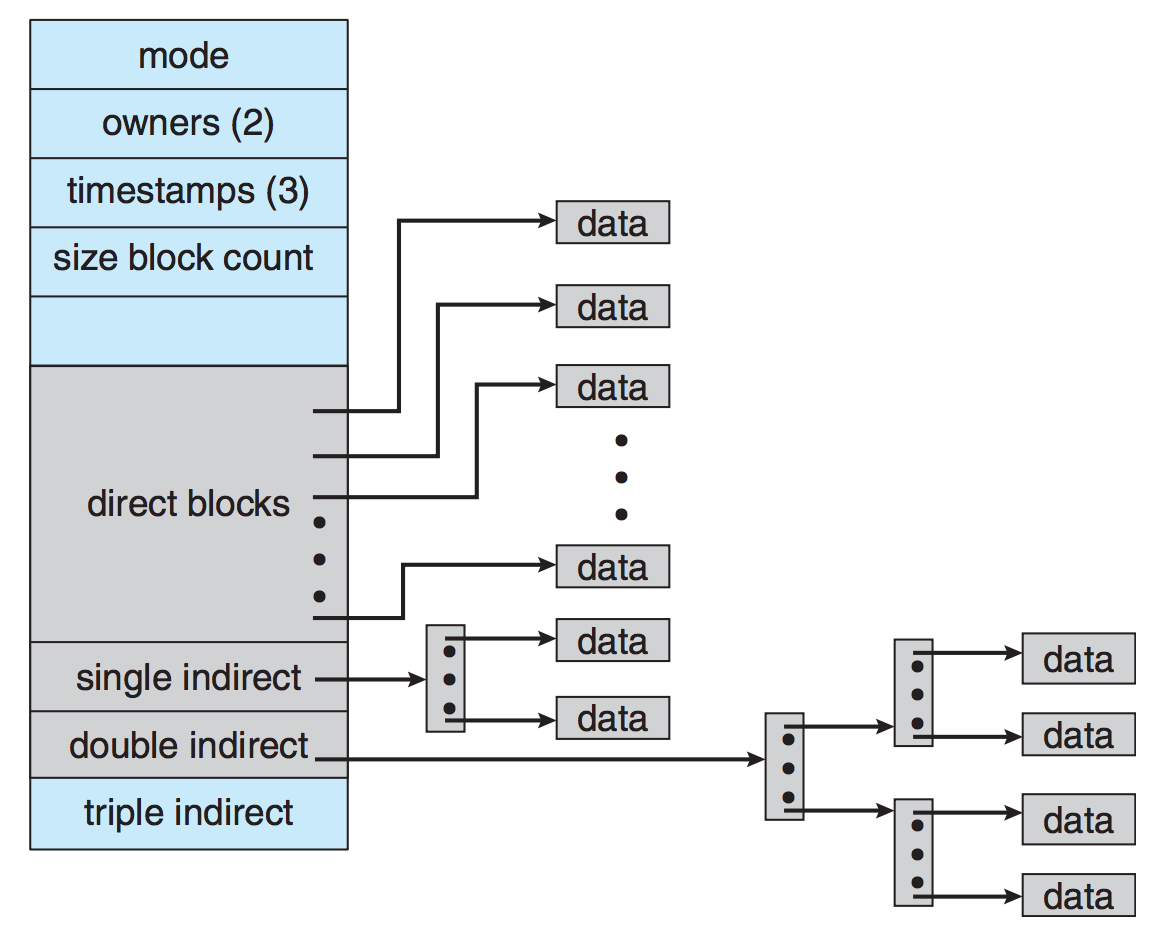
\includegraphics[width=0.6\textwidth]{images/unix-inode.png}
\end{center}

\end{frame}

\begin{frame}
\frametitle{UNIX inodes}

\begin{center}
	
\includegraphics[width=0.7\textwidth]{images/yodawg.jpg}
\end{center}

\end{frame}


\begin{frame}
\frametitle{Partial Locking}

Previously: \texttt{flock(}) to lock a file, and this locks the entire file.

Using \texttt{fcntl}, we can lock only a part of a file.

This is referred to as \alert{record locking}.

\end{frame}


\begin{frame}[fragile]
\frametitle{Partial Locking}

Locking just a part of the file allows for more concurrency!

\begin{lstlisting}[language=C]
int fcntl( int file_descriptor, int command, ... /* struct flock * flockptr */ )
\end{lstlisting}

We need to provide one \texttt{struct flock} and a \texttt{command}.


\end{frame}


\begin{frame}[fragile]
\frametitle{Struct Flock}

The \texttt{struct flock} has the following definition:
\begin{lstlisting}[language=C]
struct flock {
  short  l_type;   /* F_RDLCK, F_WRLCK, or F_UNLCK */
  short  l_whence; /* SEEK_SET, SEEK_CUR, or SEEK_END */
  off_t  l_start;  /* offset in bytes, relative to l_whence */
  off_t  l_len;    /* length, in bytes; 0 means lock to EOF */
  pid_t  l_pid;    /* returned with F_GETLK */
};
\end{lstlisting}

About \texttt{l\_type}: the types of lock are read and write.

Compatibility matrix: reads are compatible with reads; writes with nothing.

To unlock, use \texttt{F\_UNLCK}.

This is vulnerable to deadlock...

\end{frame}

\begin{frame}[fragile]
\frametitle{Struct Flock}

The \texttt{struct flock} has the following definition:
\begin{lstlisting}[language=C]
struct flock {
  short  l_type;   /* F_RDLCK, F_WRLCK, or F_UNLCK */
  short  l_whence; /* SEEK_SET, SEEK_CUR, or SEEK_END */
  off_t  l_start;  /* offset in bytes, relative to l_whence */
  off_t  l_len;    /* length, in bytes; 0 means lock to EOF */
  pid_t  l_pid;    /* returned with F_GETLK */
};
\end{lstlisting}

\texttt{l\_whence}: where does the offset begin?

It is possible for a locked region to extend past the end of the file. 

\end{frame}


\begin{frame}
\frametitle{Das war ein Befehl!}

For \texttt{command}, our choices are~\cite{apunix}:
\begin{itemize}
	\item \texttt{F\_GETLK}
	\item \texttt{F\_SETLK}
	\item \texttt{F\_SETLKW}
\end{itemize}

\end{frame}


\begin{frame}
\frametitle{Unlocking and Combining Locks}

When unlocking a region, just as for locking, you can specify what part of the file you would like to unlock. 

Partial unlocking is unusual, but why not? 

The system will combine or split locks as appropriate, 


\end{frame}

\begin{frame}[fragile]
\frametitle{Lock Usage Example}

\begin{lstlisting}[language=C]
int write_lock_file( int file_descriptor ) {

  struct flock fl;
  fl.l_type = F_WRLOCK;
  fl.l_start = 0;
  fl.l_whence = SEEK_SET;
  fl.l_len = 0;
  
  return fcntl( fd, F_SETLK, &fl );
}

int unlock_file( int file_descriptor ) {

  struct flock fl;
  fl.l_type = F_UNLCK;
  fl.l_start = 0;
  fl.l_whence = SEEK_SET;
  fl.l_len = 0;
  
  return fcntl( fd, F_SETLK, &fl );
}
\end{lstlisting}


\end{frame}

\begin{frame}[fragile]
\frametitle{Knock Knock}

Checking if a given part of a file is locked:


\begin{lstlisting}[language=C]
int fd = open ( "example.txt", O_RDONLY );
struct flock lock;

lock.l_type = F_RDLOCK;
lock.l_start = 1024;
lock.l_whence = SEEK_SET;
lock.l_len = 256;

fcntl( fd, F_GETLK, &lock );
if ( lock.l_type == F_UNLCK ) {
	/* Lock is unlocked; we may proceed */
} else if ( lock.l_type = F_WRLOCK ) {
  /* File is write locked by a different process */
  printf( "File locked by process ID %d.\n", lock.l_pid );
  return -1;
}
\end{lstlisting}

\end{frame}

\begin{frame}
\frametitle{Orders, Captain?}

Checking on things with \texttt{F\_GETLK} is really for information purposes only.

``Read the value and then whatever operation you'd like to do next'' is not
atomic.

Instead, use the command \texttt{F\_SETLK} and actually try to set the lock. 

If -1 is returned then locking was not successful.

Or, if the plan is to wait, use \texttt{F\_SETLKW} as one would expect.

\end{frame}


\begin{frame}
\frametitle{Immutability is for Cowards}

\texttt{fcntl} changes some values of the \texttt{struct lock}! 

If you wanted to re-use it you need to make sure to reset it as appropriate.

 You can use the same \texttt{struct lock} later to unlock the thing that you locked, just do so carefully.

\end{frame}


\begin{frame}
\frametitle{SPLITTERS!}
\begin{center}
	
\includegraphics[width=0.6\textwidth]{images/jpf.jpg}
\end{center}

Sometimes the name you want is taken...

 \texttt{lockf}: a simplified way of locking a file.
 
  While \texttt{fcntl} is more flexible, sometimes all we need is the simple version.

\end{frame}

\begin{frame}[fragile]
\frametitle{Locking, Simplified}

\begin{lstlisting}[language=C]
int lockf( int file_descriptor, int command, off_t length );
\end{lstlisting}

The command options can be:
\begin{itemize}
	\item \texttt{F\_LOCK} 
	\item \texttt{F\_TLOCK}
	\item \texttt{F\_ULOCK}
	\item \texttt{F\_TEST}
\end{itemize}

The length is an offset, and is based off the current position in the file. 

If zero is provided then it locks the whole file.

\end{frame}


\begin{frame}
\frametitle{Close up for the Day}

 The file is automatically unlocked when the file descriptor is closed. 
 
 And, on some systems \texttt{lockf} just calls \texttt{fcntl} but on some others they use different mechanisms. 
 
 So don't mix and match. 
 
 If you lock a file with one function, unlock it with the matching one.


\end{frame}


\begin{frame}
\frametitle{There are Rules}

It is noteworthy that both kinds of lock are ``advisory'' only.

It only is really effective if everyone involved in accessing the shared resource follows the proper protocol and checks if access is permitted or not.

Mandatory locks do exist, but are hard to use and are not recommended.

The notes link to why you shouldn't!


\end{frame}

\begin{frame}
\frametitle{I am become Lock}

We can use the very existence of a file as a way of controlling concurrency. 

For example, \texttt{git} places a file \texttt{index.lock} in a particular directory to indicate that an operation is in progress.

Thus two different \texttt{git} clients do not operate on the same repository at the same time. 

\end{frame}



\begin{frame}
\frametitle{Open Sesame?}

If we want to check, we just try to \texttt{open()} the file, but unless we are careful this can lead to a problem if two processes want to create the file.

If they both call \texttt{open}, they both might succeed. To get around this, we need to use the \texttt{flags} parameter

\end{frame}



\begin{frame}[fragile]
\frametitle{File Operations}
\begin{lstlisting}[language=C]
int open(const char *filename, int flags); 
int rename(const char *old_filename, const char *new_filename);
int remove(const char *filename); 
\end{lstlisting}

When opening a file the following flags may be used for the \texttt{flags} parameter (and can be combined with bitwise OR, the \texttt{|} operator):

{\scriptsize
\begin{tabular}{l|l}
	\textbf{Value}     & \textbf{Meaning}                                                                                 \\ \hline
	\texttt{O\_RDONLY} & Open the file read-only                                                                          \\ \hline
	\texttt{O\_WRONLY} & Open the file write-only                                                                         \\ \hline
	\texttt{O\_RDWR}   & Open the file for both reading and writing                                                       \\ \hline
	\texttt{O\_APPEND} & Append information to the end of the file                                                        \\ \hline
	\texttt{O\_TRUNC}  & Initially clear all data from the file                                                           \\ \hline
	\texttt{O\_CREAT}  & Create the file                                                                                  \\ \hline
	\texttt{O\_EXCL}   & If used with \texttt{O\_CREAT}, the caller MUST create the file; if the file exists it will fail \\
\end{tabular}
}

\end{frame}


\begin{frame}
\frametitle{Lock-File Behaviour}

Team-up \texttt{open} and \texttt{rename} to get lock-like behaviour between different programs that share nothing except a common file system.

The \texttt{open} call should be used to create the lock file, and fail if the file already exists.

If we want we can use \texttt{remove} to delete the lock file if we want to let the next process try, but there�s an alternative option: \texttt{rename}.

The \texttt{rename} function is also atomic!

To lock: change the name; to unlock, change it back!

\end{frame}


\begin{frame}[fragile]
\frametitle{Using a File as a Lock}
\begin{lstlisting}[language=C]
#include <stdio.h>
#include <stdlib.h>
#include <fcntl.h>
#include <unistd.h>
#include <sys/stat.h>
#include <sys/types.h>
#include <pthread.h>
#define NUM_THREADS 10

int lock_fd;
int shared = 0;

void* run( void* arg ) {
  int* id = (int*) arg;
  while( rename( "file.lock", "file.locked" ) == -1 ) {
    printf("Thread %d waiting.\n", *id); 
  }
  printf("Thread %d in critical section.\n", *id);
  printf("Shared incremented from %d", shared);
  shared++;
  printf(" to %d.\n", shared);
  rename("file.locked", "file.lock"); /* Unlock */

  free( arg );
  pthread_exit(NULL);
}
\end{lstlisting}

\end{frame}

\begin{frame}[fragile]
\frametitle{Using a File as a Lock}
\begin{lstlisting}[language=C]
void* writer( void* arg ) {
  /* Write data implementation not shown */
  pthread_exit(NULL);
}

int main( int argc, char** argv ) {
  lock_fd = open( "file.lock", O_CREAT | O_EXCL );  
  if (lock_fd == -1 ) {
   printf( "File creation failed.\n");
   return -1;
  }

  pthread_t threads[NUM_THREADS];
  for (int i = 0; i < NUM_THREADS; i++) {
    int * id = malloc( sizeof( int ) );
    *id = i;
    pthread_create( &threads[i], NULL, run, id );
  }
  for (int i = 0; i < NUM_THREADS; i++) {
    pthread_join( threads[i], NULL );
  }
  close( lock_fd );
  remove( "file.lock" );

  return 0;
}
\end{lstlisting}
\end{frame}


\end{document}
